\section{Introduction}
According to the world energy council, hydropower is the most flexible and
consistent of the renewable energy resources, and, at the end of 2008, the total
capacity of hydropower resources was 874 GW. Brazil is the second
country in hydropower producing and one of the world's richest countries in
water resources, motivating the development and investment in hydropower
generation. The hydropower is the most dominant across the country, and Brazil
is the second country with the highest consumption of hydropower with a 70.000
MW installed capacity, and 433 hydroelectric plants in operation.
%\begin{figure}[h!]
%	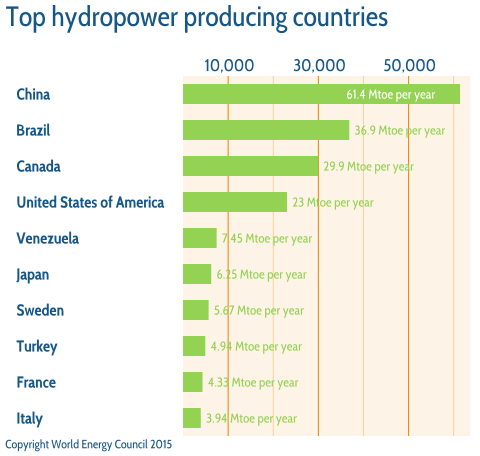
\includegraphics[width=\columnwidth]{figs/intro/graph.png}
%	\caption{Top hydropower producing countries}
%	\label{fig::cavitacao}
%\end{figure}

%O Brasil é um dos países mais ricos do mundo em recursos hídricos, facilitando
% o desenvolvimento e investimento em geração de energia a partir desse recurso. A
%energia hidráulica é a mais dominante em todo o país, e o Brasil é o segundo
%país com maior consumo de energia hidrelétrica no mundo com capacidade
%instalada de 70.000 MW, 433 usinas hidrelétricas em operação. 

In Brazil, the renovation and improvement of the built large plants is estimated
to result in a potential increase of 32.000 MW \citep{goldemberg2007energia}, a
figure that can be achieved, in large part, by the maintenance of the hydropower turbines. These turbines are constantly
exposed to abrasion and cavitation phenomena, which determine its life cycle.
%Estima-se que a reforma e melhoria das grandes usinas construídas resultariam
%em um aumento potencial de 32.000 MW \citep{goldemberg2007energia},
%número que pode ser alcançado, em grande parte, pela manutenção das turbinas
%geradoras da energia elétrica. As turbinas estão constantemente expostas aos
%fenômenos de abrasão e cavitação, os quais determinam sua vida útil.

The cavitation phenomenon is very well studied and detailed in
\cite{escaler2006detection}, which outlines their types, occurrences and
effects in the different hydraulic turbines. This physical phenomenon can cause
erosions in the hydraulic turbines, leading to water flow instability,
excessive vibrations and turbine efficiency reduction.
%O fenômeno de cavitação está muito bem estudado e detalhado em
%\cite{escaler2006detection}, onde são apresentadas seus tipos, ocorrências e os
%efeitos nas diferentes turbinas. Esse fenômeno físico pode causar erosões na
%máquina hidráulica (figura~\ref{fig::cavitacao}), gerando instabilidade de
% fluxo de água, vibrações excessivas e redução da eficiência da turbina.

\begin{figure}[h!]	
	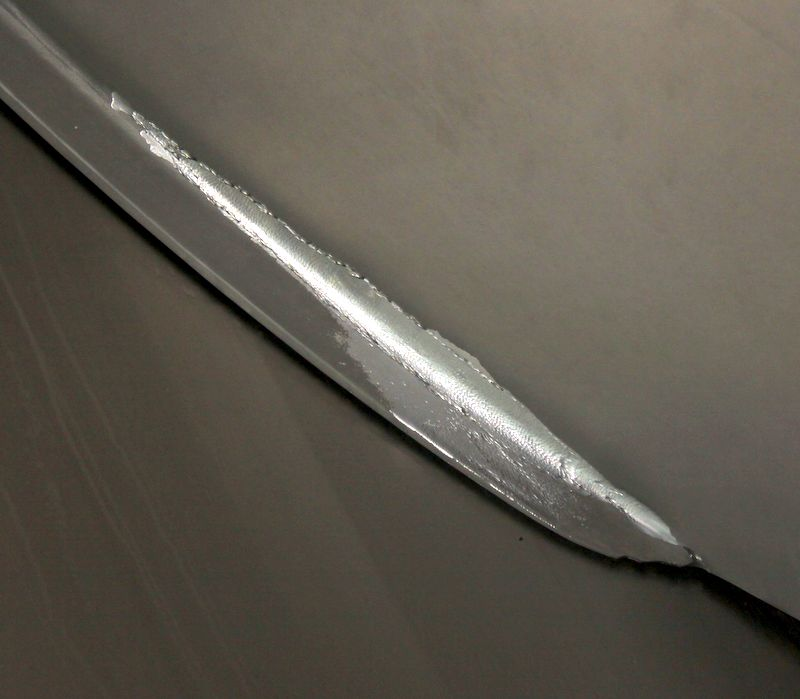
\includegraphics[width=\columnwidth]{figs/intro/cavitacao2}
	\caption{Jirau hydraulic turbine blade eroded by cavitation.}
	\label{fig::cavitacao}
\end{figure}

Hard coating techniques by thermal aspersion
are used to reduce the blade erosion from cavitation or abrasion,
and to increase its life cycle. This solution is analogous to an ink that
protects walls from environment exposure. The hard coating procedure is performed
before the hydraulic turbine installation by a robotic manipulator. The system
requires a robotic system due to high precision, requires speed, and
the harmful to health substances that are used, as propane and other gases.
Although sufficient for blade protection, the coating also has a life
cycle itself, thus it needs to be redone from time to time to ensure the
blade protection from physical phenomena.
%A fim de reduzir o desgaste da pá contra cavitação ou abrasão e aumentar a sua
%vida útil, utiliza-se a técnica de revestimento por asperção térmica, que pode
%% ser comparada com uma tinta que protege à exposição com o ambiente. O
% procedimento é realizado
%antes da instalação das pás na turbina por um robô, pois exige alta precisão
%e velocidade, além de expelir substâncias nocivas à saúde. Apesar de suficiente
% para a proteção da pá, o revestimento também tem vida útil e precisa ser refeito de tempos em tempos para
%garantir a proteção da pá contra os fenômenos físicos.

In the specific case of the Jirau hydroelectric dam, built on the Madeira
river, the number of particles that the river carries daily intensifies the
abrasion phenomena, and Rijeza, a hard coating specialized company, identified
cavitation erosion on blades, further reducing the coating life cycle.
Therefore, Jirau hydroelectric dam needs regular maintenance, which,
in the present situation, requires stoppage of the turbine, unmounting the
turbine's blades, positioning the blades for coating, coating application,
turbine assembling, and recalibration. The downtime to perform all
maintenance can takes two months, meaning a huge loss in power generation .
%No caso específico da usina hidrelétrica de Jirau, construída no rio Madeira,
%os fenômenos de abrasão são intensos devido ao grande número
%de partículas que o rio carrega diariamente, reduzindo ainda mais a vida útil
% do revestimento.
%Portanto, há a necessidade de manutenção regular, o que, na situação atual,
%exige paralização da máquina, desmontagem da turbina, posicionamento de cada pá
%na área designada ao revestimento, aplicação do revestimento, montagem da
%turbina e recalibração. O tempo de paralização para a realização de
%toda a manutenção pode levar de um a dois meses, significando uma grande perda
%na geração de energia. 

EMMA is an R\&D project by Fundação Coordenação de Projetos, Pesquisas e Estudos
Tecnológicos (COPPETEC), in partnership with Rijeza company, Agência Nacional de
Energia Elétrica (ANEEL) and Energia Sustentável do Brasil (ESBR). Its first
stage is a technical feasibility study of a robotic system to perform
coating by thermal spray on hydraulic turbine blades within the turbine
environment. The project aims to significantly reduce the downtime for hard
coating process.
%A primeira etapa do projeto EMMA, pesquisa e desenvolvimento
%realizados pela Fundação COPPETEC, em parceria com a empresa Rijeza, ANEEL e
%ESBR, é um estudo de viabilidade técnica de um sistema robótico para realizar
%revestimento por aspersão térmica de turbinas \textit{in situ}, ou seja, dentro
%do ambiente da turbina (aro câmara). O projeto tem como objetivo reduzir
%significativamente o tempo de manutenção do revestimento por ser realizado no
%ambiente confinado da turbina e, portanto, não havendo necessidade de sua
%desmontagem.

This document is divided as follows: section 2 describes, in detail, the
problem, contextualizes the reader in the Jirau environment and
describes the robot's tasks; section 3 surveys the state of the
art; section 4 describes the conceptual designs for the robot and mechanical
bases; finally, the section 5 concludes and outlines the next steps for the
EMMA project.
%Este documento está dividido da seguinte forma: a seção 2 descreve
%detalhadamente o problema, contextualiza o leitor no ambiente da usina de
%Jirau e descreve as possíveis tarefas do robô; a seção 3 faz um levantamento do
%estado da arte; a seção 4 descreve os projetos conceituais para o robô; e a
%seção 5 conclui e descreve os próximos passos para o projeto EMMA. 
